\textbf{Example}

Consider the following call:

\texttt{init(3, [2, 6, 9], [3, 1, 2], [2, 2, 3], [1, 0, 1])}

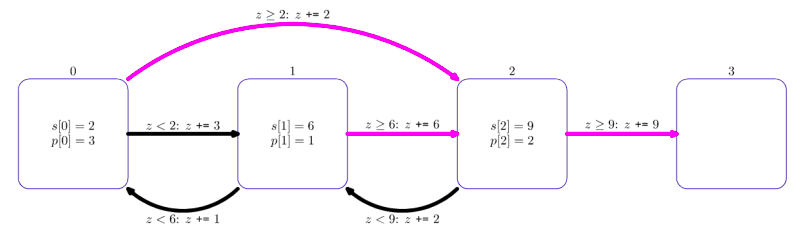
\includegraphics[scale=0.6]{1.png}

The diagram above illustrates this call. Each square shows a dungeon. For dungeons $0$, $1$ and $2$,
the values $s[i]$ and $p[i]$ are indicated inside the squares. Magenta arrows indicate where the hero
moves after winning a confrontation, while black arrows indicate where the hero moves after losing.

Let's say the grader calls \texttt{simulate(0, 1)}.

The game proceeds as follows:

\begin{center}
\renewcommand{\arraystretch}{1.5}
\begin{tabular}{|c|c|c|}
\hline
 Dungeon & Hero's strength before confrontation & Result \\
\hline
 $0$ & $1$ & Lose \\
\hline
 $1$ & $4$ & Lose \\
\hline
 $0$ & $5$ & Win \\
\hline
 $2$ & $7$ & Lose \\
\hline
 $1$ & $9$ & Win \\
\hline
 $2$ & $15$ & Win \\
\hline
 $3$ & $24$ & Game ends \\
\hline
\end{tabular}
\end{center}

As such, the procedure should return $24$.

Let's say the grader calls \texttt{simulate(2, 3)}.

The game proceeds as follows:

\begin{center}
\renewcommand{\arraystretch}{1.5}
\begin{tabular}{|c|c|c|}
\hline
 Dungeon & Hero's strength before confrontation & Result \\
\hline
 $2$ & $3$ & Lose \\
\hline
 $1$ & $5$ & Lose \\
\hline
 $0$ & $6$ & Win \\
\hline
 $2$ & $8$ & Lose \\
\hline
 $1$ & $10$ & Win \\
\hline
 $2$ & $16$ & Win \\
\hline
 $3$ & $25$ & Game ends\\
\hline
\end{tabular}
\end{center}

As such, the procedure should return $25$.